\documentclass[10pt]{book}
\usepackage[utf8]{inputenc}
%\usepackage[T1]{fontenc}
\usepackage{tgbonum}
\usepackage[english]{babel}
\usepackage{graphicx}
\usepackage{amsmath}
\usepackage{amssymb}
\usepackage{hyperref}
\usepackage{epsf}
\usepackage{float}
\usepackage{mathpazo}
\usepackage
[
a4paper,% other options: a3paper, a5paper, etc
left=2.2cm,
right=2.2cm,
top=3cm,
bottom=3cm,
]{geometry}
%\geometry{hmargin=3.5cm, vmargin=2.5cm}
\usepackage{fancyhdr}
\pagestyle{fancy}
\fancyhf{}
\rfoot{\thepage}
\renewcommand{\headrulewidth}{0pt}
\usepackage{color}
\graphicspath{{DWGs/}}
\usepackage{graphicx}
\usepackage{wrapfig}
\usepackage{graphicx}
\usepackage{multicol}
\usepackage{enumitem}
\usepackage{xcolor}
\usepackage{framed}
\definecolor{shadecolor}{RGB}{139, 231, 3}

\usepackage{tcolorbox}
\definecolor{mycolor}{rgb}{0.122, 0.435, 0.698}

\newtcbox{\mb}{nobeforeafter,colframe=mycolor,colback=mycolor!10!white,boxrule=0.5pt,arc=4pt,
  boxsep=0pt,left=6pt,right=6pt,top=3pt,bottom=3pt,tcbox raise base}

\usepackage{eso-pic}
\newcommand\BackgroundPic{%
\put(-50,-0){%
\parbox[b][\paperheight]{\paperwidth}{%
\vfill
\centering
\includegraphics[height=\paperheight,%
keepaspectratio]{DWGs/cover.png}%
\vfill
}}}

\usepackage{anyfontsize}
\usepackage{t1enc}

\makeatletter
\def\thickhrulefill{\leavevmode \leaders \hrule height 1ex \hfill \kern \z@}
\def\@makechapterhead#1{%
  \vspace*{10\p@}%
  {\parindent \z@ \raggedleft \reset@font
            \scshape \@chapapp{} \thechapter
        \par\nobreak
        \interlinepenalty\@M
    \Huge \bfseries #1\par\nobreak
    %\vspace*{1\p@}%
    \hrulefill
    \par\nobreak
    \vskip 100\p@
  }}
\def\@makeschapterhead#1{%
  \vspace*{10\p@}%
  {\parindent \z@ \raggedleft \reset@font
            \scshape \vphantom{\@chapapp{} \thechapter}
        \par\nobreak
        \interlinepenalty\@M
    \Huge \bfseries #1\par\nobreak
    %\vspace*{1\p@}%
    \hrulefill
    \par\nobreak
    \vskip 100\p@
  }}

\begin{document}


\begin{titlepage}

\AddToShipoutPicture*{\BackgroundPic}

\ \\[4cm]

{\sffamily \color{white}
\begin{center}
\fontsize{56}{10}\selectfont F l u i d T o o l b o x
\end{center}
}

\vfill


{\fontsize{20}{20}\color{white}\sffamily Science Docs \hfill\color{white} Kamila Zdybał}

\end{titlepage}


\thispagestyle{empty}

\ \\[12cm]
\begin{flushright}%
\includegraphics[width = 100mm]{cover.png}

\ \\[0.5cm]

\textit{About the cover photo:} view from the coast of the Cres island in Croatia, October 2016.

\ \\[0.1cm]

Photo by: J. Aleksanderek
\end{flushright}
\newpage

\thispagestyle{empty}
\begin{center}
    
\vspace*{4cm}

\includegraphics[width = 80mm]{ex_libris_arduino.png}

\vspace*{2cm}

Copyright \textcopyright \, K. Zdybał, 2018

For more projects similar to this one

visit me on GitHub: \verb|@camillejr|

\verb|camillejr.github.io/science-docs/|

To contact me personally drop me a line at:

\verb|kamilazdybal@gmail.com|

\vspace*{2cm}

\verb|Fluid Toolbox|

\verb|version 1.0|
\end{center}


\setlength{\parskip}{0.6em}
\setlength{\parindent}{0cm}




% Fluid Toolbox content

\chapter{Circulation}



Circulation is defined as:

\begin{equation}
\Gamma = \oint_C \vec{\upsilon} \cdot \vec{dl}
\end{equation}

The dot operation gives a scalar which is expressing "how much" in the direction of the other vector is this vector.

\begin{figure}[H]
\centering\includegraphics[width=5cm]{circulation_dot_prod}
\caption{Dot product of two vectors.}			
\label{fig:learning_curve}
\end{figure}

When they are $\perp$, the dot product is zero.

In the concept of circulation, you ask "how much" at any point on the curve $C$ the velocity vector at that point is in the direction of the curve's geometry. Now, that doesn't yet sound as something to do with "circulating". For the moment, I would think that it's more of an "on-trackness". Something, that in real world would be for instance the measure of how much the vehicle's velocity is in the direction of the road geometry.

But then you realise an important detail of "$\circ$" on the integral symbol, which means that the curve should be a closed curve - a loop.

When you perform integration, which means summing up every little $\vec{\upsilon} \cdot \vec{dl}$ as you go around the loop, you count "how much" at every point on the loop, the velocity vector at these points is in the direction of the loop's geometry (at these points).

If we were to place a small particle at some starting point $P$ on the loop, the circulation would tell us "how much" the velocity field which this particle is subjected to, is tending to move that particle around the loop.

It can be very intuitive when you take a look at these two pictures:



It's no surprise that when the velocity is everywhere perpendicular to the loop's geometry, the circulation around the loop is zero. If you were to place a particle at any point on the loop, such velocity field would act to immediately displace the particle off the loop. Therefore, the particle would have no way of "circulating" around the loop.

On the other extreme is the case when the velocity field is everywhere tangent to the loop's geometry. Anywhere the particle goes on the loop, the velocity at that point would act to keep the particle moving around the loop.

Questions:

\begin{enumerate}
\item Why closed loop? Would it have any meaning if we calculated circulation along any general spline?

\item How to chose loops so that the circulation we calculate is of the most meaning to us?

\item What does the zero, positive, negative circulation mean?

\item Can circulation be infinite?
\end{enumerate}



\chapter{Vorticity}


\begin{enumerate}
\item Why is vorticity concept needed? Isn't it something kind of like circulation?

\end{enumerate}


\chapter{Stoke's Theorem}

\input{stokes_theorem/stokes_theorem.tex}




\begin{thebibliography}{50}
\end{thebibliography}
\end{document}